%插入样式内容
\documentclass[12pt]{article}
%%---------------------------------------------------------------------
% packages
% geometry
\usepackage{color}
\usepackage{geometry}
% font
\usepackage{fontspec}
\defaultfontfeatures{Mapping=tex-text}  %%如果没有它,会有一些 tex 特殊字符无法正常使用,比如连字符。
\usepackage{xunicode,xltxtra}
\usepackage[BoldFont,SlantFont,CJKnumber,CJKchecksingle]{xeCJK}  % \CJKnumber{12345}: 一万二千三百四十五
\usepackage{CJKfntef}  %%实现对汉字加点、下划线等。
\usepackage{pifont}  % \ding{}
% math
\usepackage{amsmath,amsfonts,amssymb}
% color
\usepackage{color}
\usepackage{xcolor}
\definecolor{EYE}{RGB}{199,237,204}
\definecolor{FLY}{RGB}{128,0,128}
\definecolor{ZHY}{RGB}{139,0,255}
% graphics
\usepackage[americaninductors,europeanresistors]{circuitikz}
\usepackage{tikz}
\usetikzlibrary{positioning,arrows,shadows,shapes,calc,mindmap,trees,backgrounds}  % placements=positioning
\usepackage{graphicx}  % \includegraphics[]{}
\usepackage{subfigure}  %%图形或表格并排排列
% table
\usepackage{colortbl,dcolumn}  %% 彩色表格
\usepackage{multirow}
\usepackage{multicol}
\usepackage{booktabs}
% code
\usepackage{fancyvrb}
\usepackage{listings}
% title
\usepackage{titlesec}
% head/foot
\usepackage{fancyhdr}
% ref
\usepackage{hyperref}
% pagecolor
\usepackage[pagecolor={EYE}]{pagecolor}
% tightly-packed lists
\usepackage{mdwlist}

\usepackage{styles/iplouccfg}
\usepackage{styles/zhfontcfg}
\usepackage{styles/iplouclistings}
\usepackage{listings} 
\usepackage{hyperref}
\usepackage{color,framed}
%\usepackage{styles/pythonhighlight}
%\usepackage{graphicx}
%%---------------------------------------------------------------------
% settings
% geometry
\geometry{left=2cm,right=1cm,top=2cm,bottom=2cm}  %设置 上、左、下、右 页边距
\linespread{1.5} %行间距
% font
\setCJKmainfont{Adobe Kaiti Std}
%\setmainfont[BoldFont=Adobe Garamond Pro Bold]{Apple Garamond}  % 英文字体
%\setmainfont[BoldFont=Adobe Garamond Pro Bold,SmallCapsFont=Apple Garamond,SmallCapsFeatures={Scale=0.7}]{Apple Garamond}  %%苹果字体没有SmallCaps
\setCJKmonofont{Adobe Fangsong Std}
% graphics
\graphicspath{{figures/}}
\tikzset{
    % Define standard arrow tip
    >=stealth',
    % Define style for boxes
    punkt/.style={
           rectangle,
           rounded corners,
           draw=black, very thick,
           text width=6.5em,
           minimum height=2em,
           text centered},
    % Define arrow style
    pil/.style={
           ->,
           thick,
           shorten <=2pt,
           shorten >=2pt,},
    % Define style for FlyZhyBall
    FlyZhyBall/.style={
      circle,
      minimum size=6mm,
      inner sep=0.5pt,
      ball color=red!50!blue,
      text=white,},
    % Define style for FlyZhyRectangle
    FlyZhyRectangle/.style={
      rectangle,
      rounded corners,
      minimum size=6mm,
      ball color=red!50!blue,
      text=white,},
    % Define style for zhyfly
    zhyfly/.style={
      rectangle,
      rounded corners,
      minimum size=6mm,
      ball color=red!25!blue,
      text=white,},
    % Define style for new rectangle
    nrectangle/.style={
      rectangle,
      draw=#1!50,
      fill=#1!20,
      minimum size=5mm,
      inner sep=0.1pt,}
}
\ctikzset{
  bipoles/length=.8cm
}
% code
\lstnewenvironment{VHDLcode}[1][]{%
  \lstset{
    basicstyle=\footnotesize\ttfamily\color{black},%
    columns=flexible,%
    framexleftmargin=.7mm,frame=shadowbox,%
    rulesepcolor=\color{blue},%
%    frame=single,%
    backgroundcolor=\color{yellow!20},%
    xleftmargin=1.2\fboxsep,%
    xrightmargin=.7\fboxsep,%
    numbers=left,numberstyle=\tiny\color{blue},%
    numberblanklines=false,numbersep=7pt,%
    language=VHDL%
    }\lstset{#1}}{}
\lstnewenvironment{VHDLmiddle}[1][]{%
  \lstset{
    basicstyle=\scriptsize\ttfamily\color{black},%
    columns=flexible,%
    framexleftmargin=.7mm,frame=shadowbox,%
    rulesepcolor=\color{blue},%
%    frame=single,%
    backgroundcolor=\color{yellow!20},%
    xleftmargin=1.2\fboxsep,%
    xrightmargin=.7\fboxsep,%
    numbers=left,numberstyle=\tiny\color{blue},%
    numberblanklines=false,numbersep=7pt,%
    language=VHDL%
    }\lstset{#1}}{}
\lstnewenvironment{VHDLsmall}[1][]{%
  \lstset{
    basicstyle=\tiny\ttfamily\color{black},%
    columns=flexible,%
    framexleftmargin=.7mm,frame=shadowbox,%
    rulesepcolor=\color{blue},%
%    frame=single,%
    backgroundcolor=\color{yellow!20},%
    xleftmargin=1.2\fboxsep,%
    xrightmargin=.7\fboxsep,%
    numbers=left,numberstyle=\tiny\color{blue},%
    numberblanklines=false,numbersep=7pt,%
    language=VHDL%
    }\lstset{#1}}{}
% pdf
\hypersetup{%pdfpagemode=FullScreen,%
            pdfauthor={Haiyong Zheng},%
            pdftitle={Title},%
            CJKbookmarks=true,%
            bookmarksnumbered=true,%
            bookmarksopen=false,%
            plainpages=false,%
            colorlinks=true,%
            citecolor=green,%
            filecolor=magenta,%
            linkcolor=cyan,%red(default)
            urlcolor=cyan}
% section
%http://tex.stackexchange.com/questions/34288/how-to-place-a-shaded-box-around-a-section-label-and-name
\newcommand\titlebar{%
\tikz[baseline,trim left=3.1cm,trim right=3cm] {
    \fill [cyan!25] (2.5cm,-1ex) rectangle (\textwidth+3.1cm,2.5ex);
    \node [
        fill=cyan!60!white,
        anchor= base east,
        rounded rectangle,
        minimum height=3.5ex] at (3cm,0) {
        \textbf{\thesection.}
    };
}%
}
\titleformat{\section}{\Large\bf\color{blue}}{\titlebar}{0.1cm}{}
% head/foot
\setlength{\headheight}{15pt}
\pagestyle{fancy}
\fancyhf{}

\chead{\color{black!50!green}Cifar10 And MNIST}

%\lfoot{\color{blue!50!green}Dai Jialun}
\cfoot{\color{blue!50!green}\href{http://vision.ouc.edu.cn/~zhenghaiyong}{CVBIOUC}}
\rfoot{\color{blue!50!green}$\cdot$\ \thepage\ $\cdot$}
\renewcommand{\headrulewidth}{0.4pt}
\renewcommand{\footrulewidth}{0.4pt}


%%---------------------------------------------------------------------
\begin{document}
%%---------------------------------------------------------------------
%%---------------------------------------------------------------------
% \titlepage
\title{\vspace{-2em} 使用Caffe进行图像分类的流程\\
\normalsize{}}
\author{Wu Bin}
\date{\vspace{-0.7em} \today \vspace{-0.7em}}
%%---------------------------------------------------------------------
\maketitle\thispagestyle{fancy}
%%---------------------------------------------------------------------
\maketitle
%\tableofcontentsG
\section{创建训练集}
在测试阶段我们选择的训练集是CIFAR-10,共有60000张图像,其中有10000张为测试图像,这个分为10类,详细的介绍在戴嘉伦的github上有详细的介绍。

其实在拿到一个数据集后,一般是包含两部分的,一是图像本身,二是图像中包含label数据。有了训练集以后我们要把它转换成Caffe可以读取的数据格式,主要有Lmdb和LevelDB两种形式。

先说LevelDB,他是一个由Google实现的非常高效的Key-Value数据库,支持十亿级别的数据量。主要归功于LSM算法使得它在非常大的数量级别下还有非常高的性能。

LMDB的全称是Lightning Memory-Mapped Database,闪电般的内存映射数据库。它文件结构简单,一个文件夹,里面一个数据文件,一个锁文件。数据随意复制,随意传输。它的访问简单,不需要运行单独的数据库管理进程,只要在访问数据的代码里引用LMDB库,访问时给文件路径即可。

它们都是键/值对(Key/Value Pair)嵌入式数据库管理系统编程库。虽然lmdb的内存消耗是leveldb的1.1倍,但是lmdb的速度比leveldb快10\%至15\%,更重要的是lmdb允许多种训练模型同时读取同一组数据集。因此lmdb取代了leveldb成为Caffe默认的数据集生成格式。

对于CIFAR-10数据集,Caffe通过其example下的“create\_cifar10.sh”脚本对data目录下的二进制的Cifar数据集转换成lmdb格式。其中主要用到了“convert\_cifar\_data.cpp”这个程序,这个程序目前还没有看明白。
当然如果数据集是自己的数据集的话,可以通过caffe\_root/examples/imagenet下的“create\_imagenet.sh”脚本将自有的图片和Label文件转化为lmdb格式,不过这个目前还在测试中。



\section{对训练集进行训练}

在选定CIFAR-10作为训练集的情况下, 可以直接使用Caffe提供的model进行训练,CIFAR-10 模型是一个由卷积层、池层、修正线性单元和一个在最顶层的局部对比度归一化的线性分类器组成的卷积神经网络。并且这个模型已经在 CAFFE\_ROOT/examples/cifar10下的“cifar10\_quick\_train\_test.prototxt”和“cifar10\_full\_train\_test.prototxt”给定了。

在训练的过程中,只要使用对应的model对测试集进行训练就好了。

\begin{lstlisting}
cd $CAFFE_ROOT
./examples/cifar10/train_full.sh
\end{lstlisting}

通过阅读“train\_full.sh”,可以知道脚本主要使用了 \mcode{caffe train --solver=examples/cifar10/cifar10_full_solver.prototxt}



\subsection{MNIST介绍}
MNIST数据集是手写数字图像,其训练集有60000张图像,测试集有10000张图像。这只是一个更大的数据集NIST的一个子集。这些数字图像已经经过尺寸的规范化与在图像的置中心处理。

这个数据集适合一些人想用学习技术以及模式识别方法来处理真实世界的数据,而且不需要花太多功夫在预处理和格式化方面的工作上。

这个数据集总共有4个文件:
\begin{itemize}
\item \textbf{{\footnotesize{train-images-idx3-ubyte.gz}}} {\footnotesize{training set images (9912422 bytes)}} 
\item \textbf{{\footnotesize{train-labels-idx1-ubyte.gz}}} {\footnotesize{training set labels (28881 bytes)}} 
\item \textbf{{\footnotesize{t10k-images-idx3-ubyte.gz}}} {\footnotesize{test set images (1648877 bytes)}} 
\item \textbf{{\footnotesize{t10k-labels-idx1-ubyte.gz}}} {\footnotesize{test set labels (4542 bytes)}}
\end{itemize}

在NIST中的手写数字图像,都为灰度保真图,而且经过规范化处理,图像大小为28$\times$28。

MNIST数据集是由NIST的Special Database 3 (SD3)和Special Database 1(SD1)所组成,二者包含了手写数字的二值图像。NIST中最初将SD-3作为训练集,SD-1作为测试集。然而,SD-3比SD-1更清晰,更容易识别。主要是因为SD-3是从Census Bureau的员工处收集的,而SD-1是从高中生处收集的。从学习实验中得出可靠的结论要求结果与训练集的选择无关,并且测试样本是完整数据集。因此,必须通过混合NIST数据集来建立一个全新的数据集。

MNIST训练集是由SD-3的30000张图像和SD-1的300000张图像组成。测试集是由SD-3的5000张图像和SD-1的5000张图像组成。训练集中所包含的图像是从大约250个人中收集到的。基本可以判定训练集与测试集的数字是不同的人所写的。

SD-1是由500个不同的人所写的58527张数字图像。在SD-1中,数据是杂乱无章地排列的。这个排列方式与SD-3不同,在SD-3中每个人所写的数字图像是按序列排列的。我们可用人工方法来分辨SD-1的数字图像由哪个人缩写。我们将SD-1分为两部分:由前250个人所写的数字图像放在训练集中,剩下的250个人所写数字放在测试集中。因此,我们有了两个子集,每个子集有大约30000张图像。新的训练集从SD-3中的\#0开始提取图像30000张图像,与之前SD-1中一个子集的30000张图像合并,组成一个60000张的训练集。与其相似,新的测试集是由SD-3中的\#35000开始提取图像,与之前SD-1中另一个子集的图像合并,组成一个大的测试图像。但是在这里只需要测试集中的10000张测试图像(从SD-1中的5000张图像和从SD-3中的5000张图像)。当然,60000张的训练图像也是完全可用的。


\subsection{MNIST数据库格式}

数据存储在一个用来存放向量和多维矩阵的文件格式中。MNIST数据库主要包含四个文件:{\footnotesize{train-images-idx3-ubyte.gz}},{\footnotesize{train-labels-idx1-ubyte.gz}},{\footnotesize{t10k-images-idx3-ubyte.gz}},{\footnotesize{t10k-labels-idx1-ubyte.gz}}。在Caffe中,用{\footnotesize{get\_mnist.sh}}自动获取的数据集就是上述形式。训练集包含了60000张图像,测试集包含了10000张图像。

\begin{figure}[!ht]
  \centering 
  \subfigure[]{ 
 %   \label{fig: } %% label for first subfigure 
    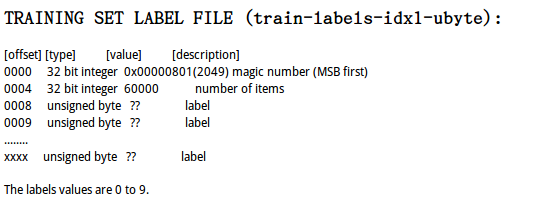
\includegraphics[width=0.31\textwidth]{mnist1}} 
  \subfigure[]{ 
 %   \label{fig: result1: b} %% label for second subfigure 
    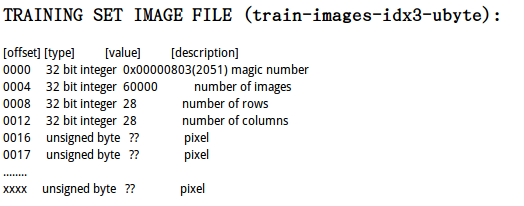
\includegraphics[width=0.3\textwidth]{mnist2}} 
  \caption{MNIST数据库训练集内容}
  \label{fig: } %% label for entire figure 
\end{figure}

在MNIST数据库中,图像数据以上述形式存储。如果要查看图像,需要经过程序的变换,转换成可打开与显示的图像格式。如图Figure~\ref{fig:mnist}。
\begin{figure}[!ht]
  \centering 
  \subfigure[]{ 
 %   \label{fig: } %% label for first subfigure 
    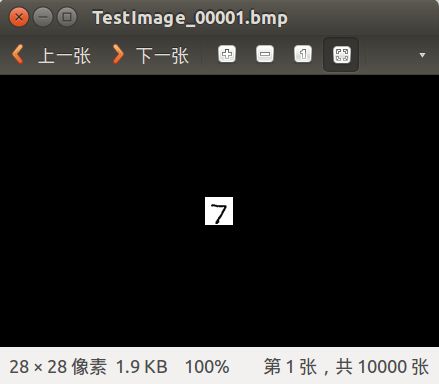
\includegraphics[width=0.3\textwidth]{mnist_example1}} 
  \subfigure[]{ 
 %   \label{fig: result1: b} %% label for second subfigure 
    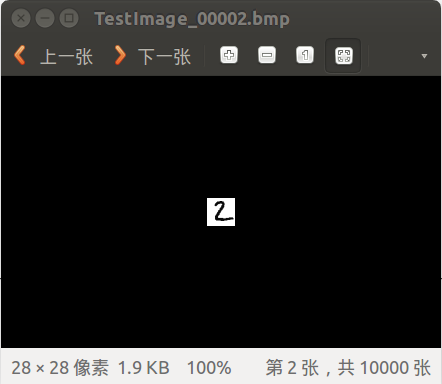
\includegraphics[width=0.3\textwidth]{mnist_example2}} 
  \caption{One image in MNIST}
  \label{fig:mnist} %% label for entire figure 
\end{figure}
%%---------------------------------------------------------------------
\end{document}
